\documentclass{article}
\usepackage{graphicx}
\usepackage{epsfig}
%\usepackage{pdflatex}
\title {SuperBigBite Data Acquisition Implementation}
\author{Alexandre Camsonne}

\begin{document}
\section{Introduction}
\subsection{CODA}
\subsubsection{Introduction}
Jefferson Laboratory is using the Cebaf Online Data Acquisition system for data taking.
CODA is based on a main server interacting with a database in which all the DAQ components update their status . The readout crates host a single board computer running a Read Out Controller (ROC) program which controls and reads out the data from the electronics. The ROCs send the data through a standard network link usually ethernet to a computer running the Event Builder program, which uses the data from the ROC to check synchronization and build the event. Finally the event is sent to the Event Recorder which puts the event into a file on the hard drive of the computer.
\subsubsection{CODA Hardware}
In addition to the software a set of harware components specific to CODA is used in order to keep ensure event synchronization between all the components each crate has a trigger interface ( TI board ) which sends the trigger signal to the ROC program for the read out of the data. All the TI are linked to a trigger supervisor board which takes the triggers and sends them to the TI while monitoring the status of each TI to keep all the crates synchronized and generates a Level 1 accept and Level 2 accept for the read out modules. The TS also takes as input the front end busy of the modules to inhibit the triggering if one module is not ready insuring synchronization between the modules.
This allows the TS module to buffering if the front-end has the capability. The triggers and read out are then decorrelated which improve the deadtime since a module can take triggers while being readout asynchronously. The TS has a setting of the maximum of events which can be in the buffer it is set to the smallest buffer available on the electronics ( usually 5 for fastbus ). Since in this mode modules can potentially get out of synchronization, a synchronization event is set so that when a certain number of triggers is processed, the TS will disable the triggers to empty the FIFO. If there any remaining events in the FIFO a warning issue would be issued and the FIFOs would be cleared resynchronizing the modules.
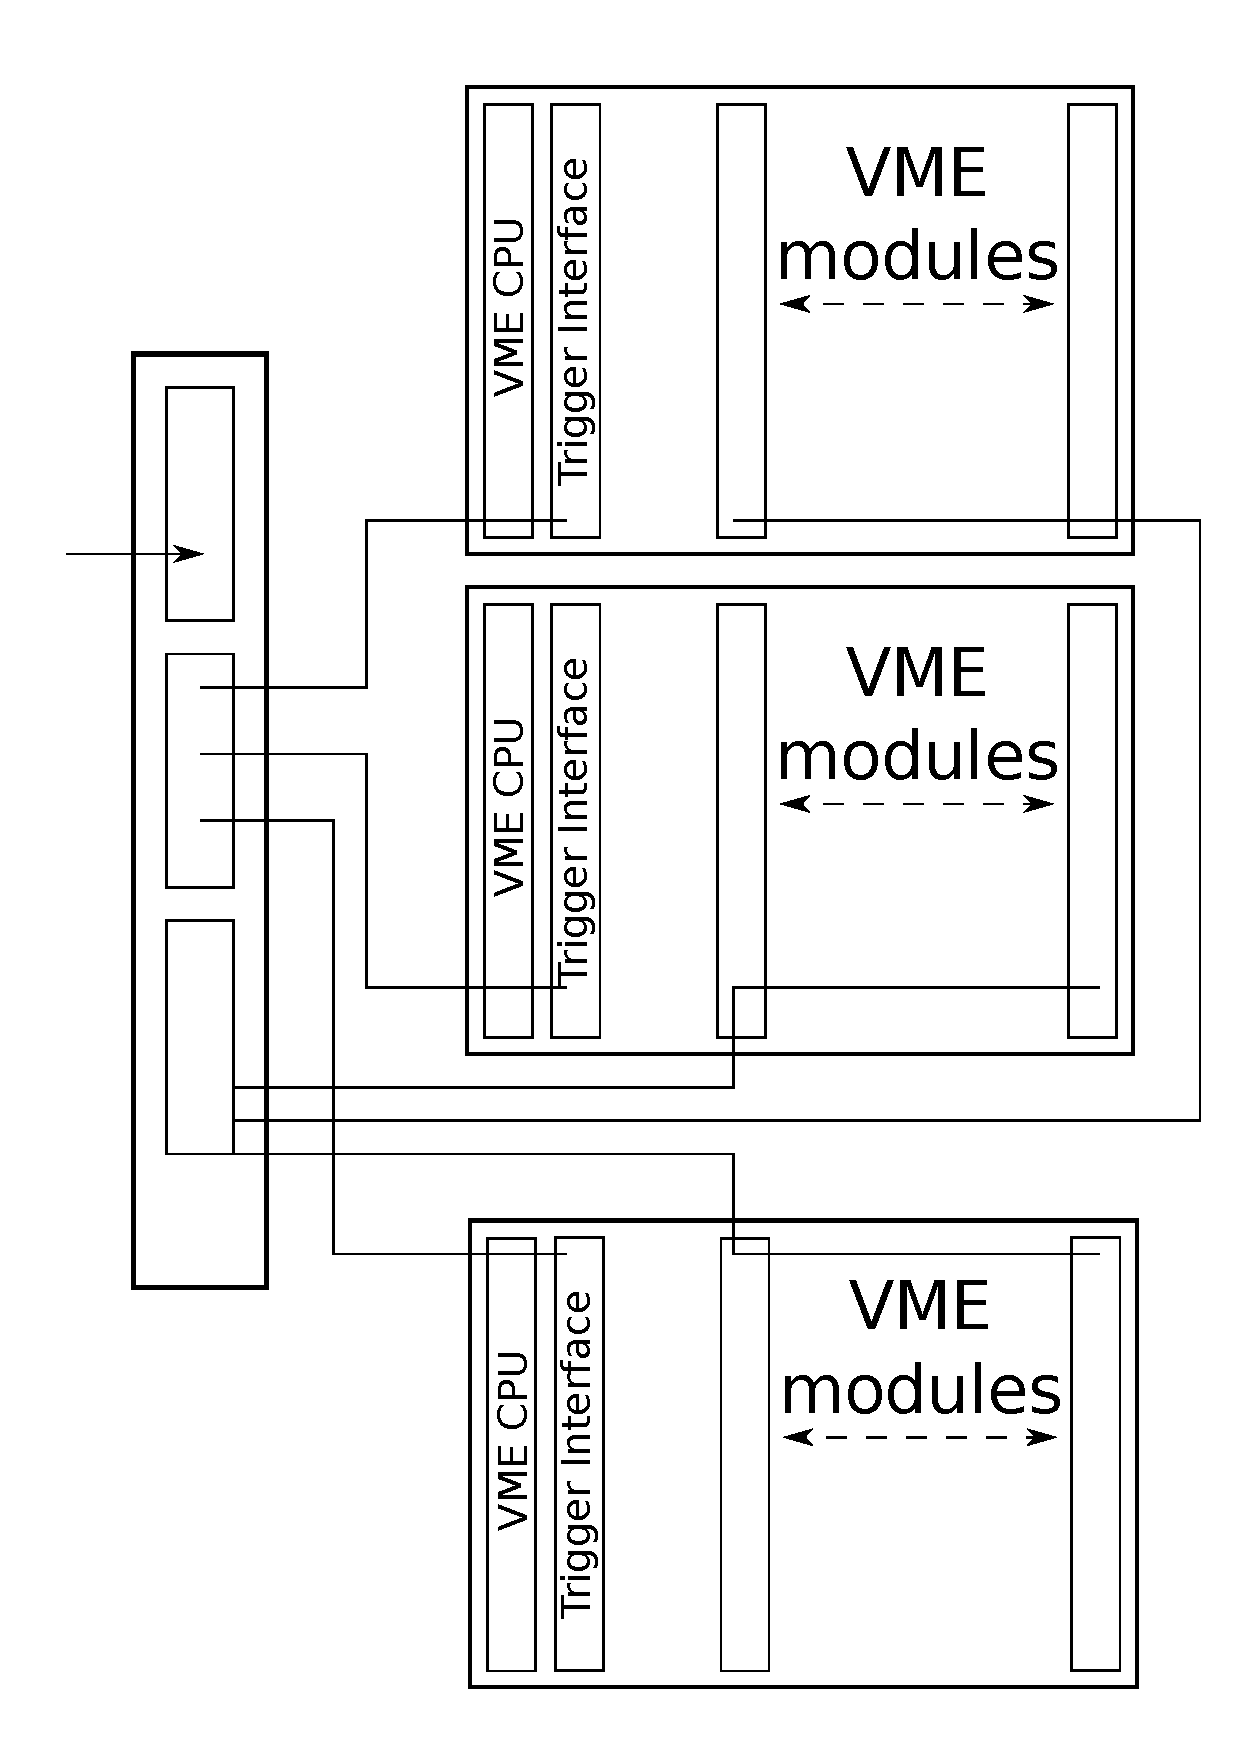
\includegraphics[scale=0.55]{figs/TS.pdf}\\
  

\section{Electronics}
\section{GEM readout}
The GEM readout is carried out by the APV25 chip. It a pipelined ASICs with 128 channels and pipeline depth of 192 samples sampling at 40 MHz. When a trigger is issued the corresponding cells are frozen until they are readout while the other cells are still being used reducing the dead time.
For each trigger all the data of 128 channels are transfered at 40 MHz rate in a multiplexed analog format. Adding some header and event informations 141 words are transmitted for each trigger which gives a transfer time of $141x25 ns = 3.6 \mu s $. In case of high background several consecutives time samples can be sent in order to detect pile up, we plan to read 3 samples which gives a transfer time of 10.8 $\mu s$. This allows deadtimeless operation for rates up to 90 KHz. The readout planned to be use the the INFN Multi Purpose Digitizer (MPD), it is a VME board with a 200 MHz FADC and signals to control the APV setup and readout. 


\section{Pipelined electronics, HCAL trigger}
The hadron calorimeter will be read out by the JLAB pipelined electronics.
The central module for this system is the JLAB FADC250, a 16-channel 12-bit FADC sampling at 250~MHz. The input signals are continuously recorded into the memory with a memory depth up to 8 us. The system is thus dead timeless as long as the trigger is generated before the memory rolls over and the event of interest is overwritten.
The Flash ADC has two separated data path.
The first one uses the new high speed serialized VME standard called VME switched Serial (VXS).
It allows full duplex point to point connection at up to 2.5 Gbps per lane using the backplane central connector.
Currently the FADC is using two VXS lanes giving 5 Gbps of bandwidth.
This allows to transfer a 16 bit word from each FADC to a Crate Trigger Processor (CTP) board every 4~ns.
Each FADC being connected to The CTP via a 5 Gbps link, the CTP uses up to 16 FADC words from each FADC to form a 32-bit word every 4~ns which can be a lower resolution sum of all the channels or a bit pattern of the channel hit for example.
The CTP board then sends the processed signals to a Sub-System Processor (SSP) board via a 10 Gbps optical link which puts together all the data from individual crates and computes the associated quantities which will be used in the trigger.
All the SSP boards send their processed information to a Global Trigger Processor (GTP) which makes the L1 trigger.
The GTP sends the trigger to the Trigger Supervisor (TS) which makes sure the system is ready to accept a trigger and sends the accepted signal to the Trigger Distribution boards in the VXS crates which are linked to the Trigger Interface boards in each crates via optical link as represented in Fig.\ref{fig:pipeline_daq}.
The trigger and synchronization clock signals will then be sent back to individual crates and payload modules through Trigger Interface/Distribution (TID) boards and Signal Distribution (SD) boards which distributes the signals to the electronics such as the FADC.
Once a trigger is generated, the full resolution data which is still in the pipeline is readout out using the VME320 protocol at an average data rate of 200 MB/s.
The Flash ADC can run in different modes, it can either transfer all the samples of the waveform which can be useful to study pileup effect and background or process the data to give an integral over the length of the pulse.

\begin{figure}
  \centering
  % Requires \usepackage{graphicx}
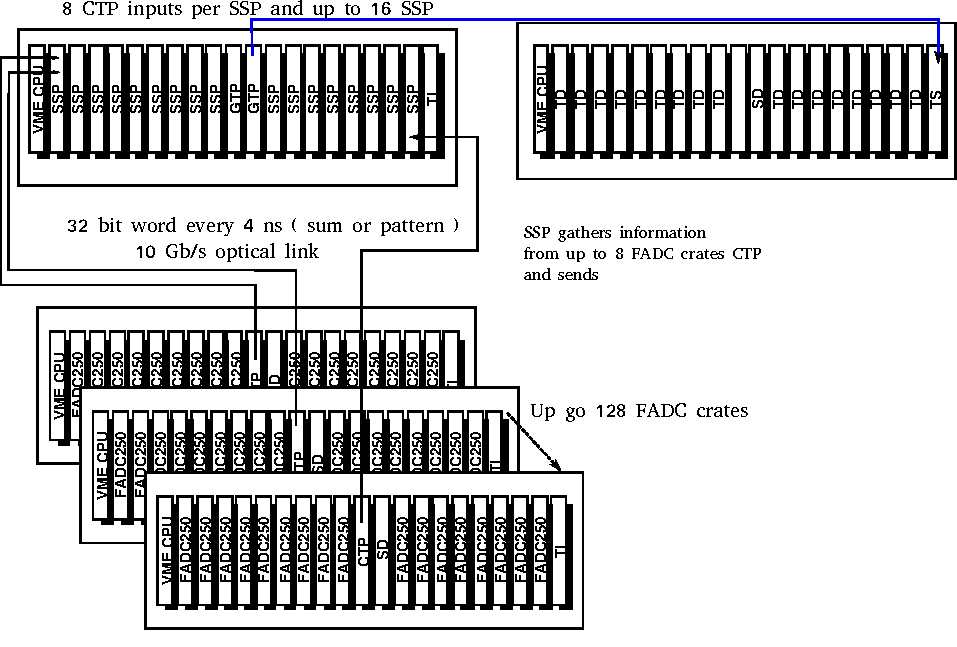
\includegraphics[width=\textwidth]{figs/TriggerPipeline.pdf}\\
  \caption{Standard Triggering scheme using the JLAB pipeline electronics}\label{fig:pipeline_daq}
\end{figure}

The CTP having all the amplitude of all the calorimeter, it can compute all the sums of adjacent blocks.
A sum of 3$\times$3 blocks was implemented.
In order to reduce the number of triggers coming from the background this summing approach is chosen to improve the online pion rejection.
A sum over 1 central block and 6 surrounding blocks can be implemented in the same way as the HPS scheme.

\begin{figure}
  \centering
  % Requires \usepackage{graphicx}
 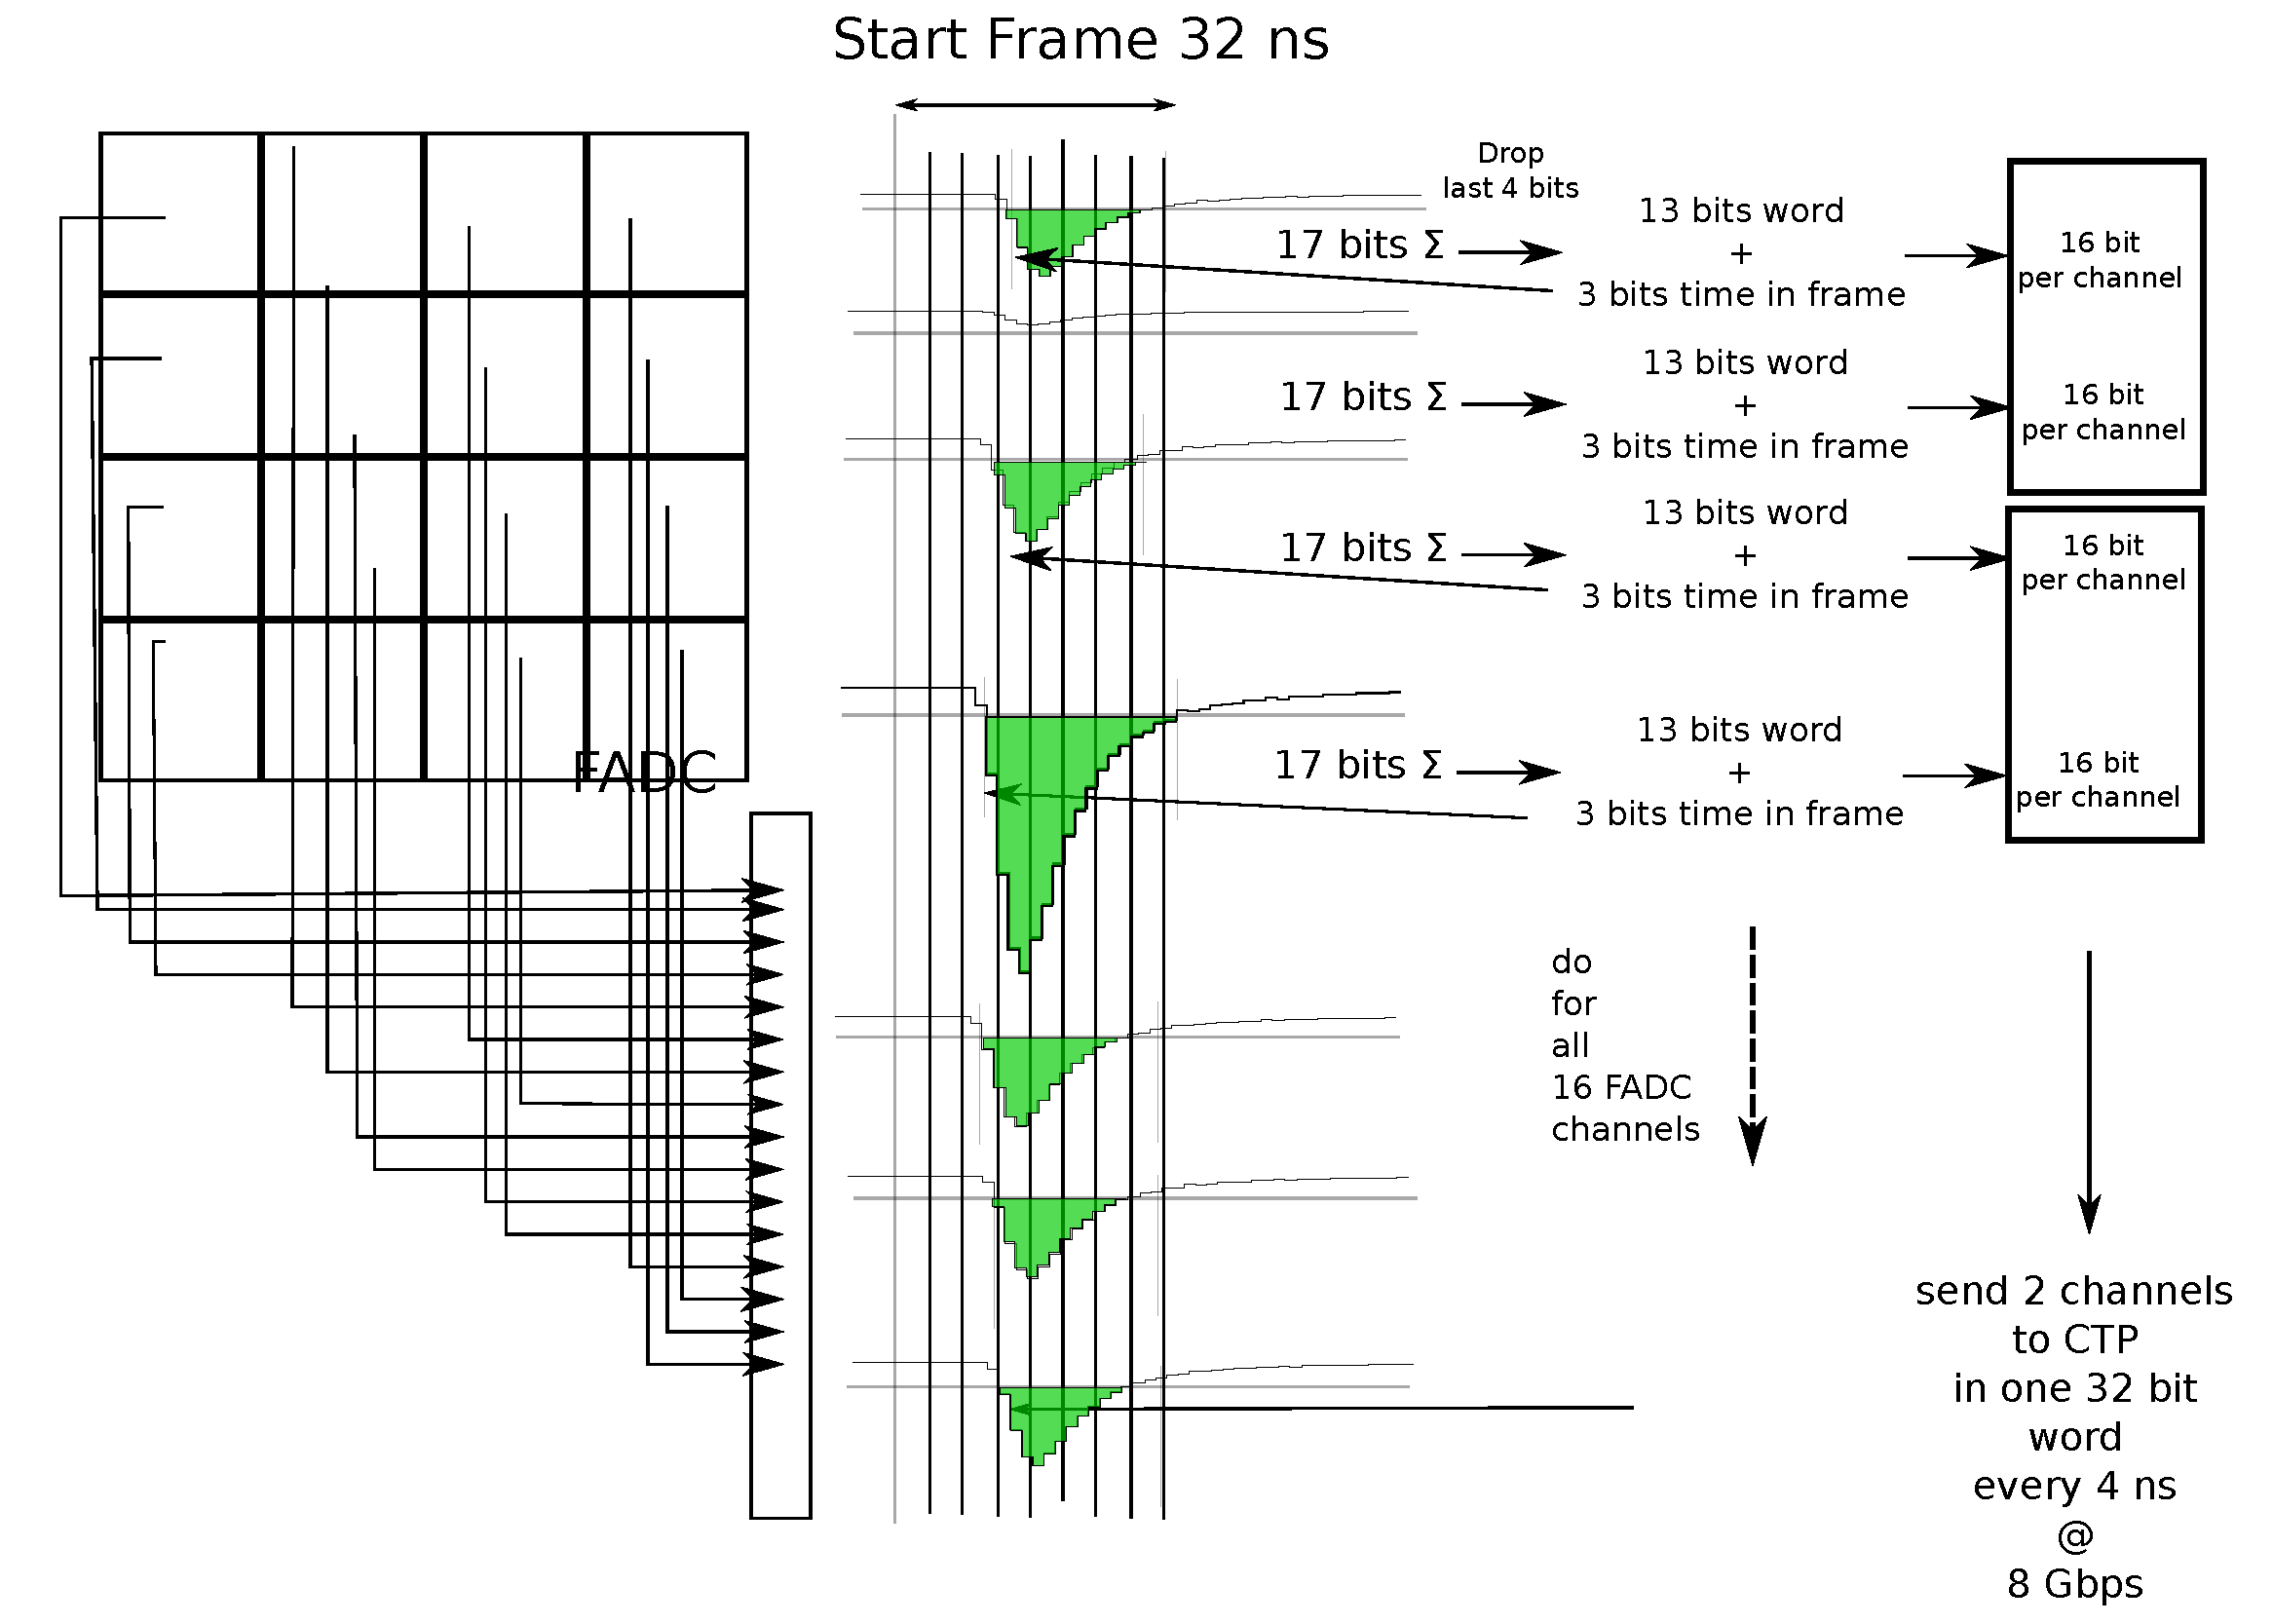
\includegraphics[width=\textwidth]{figs/CaloTrigger.pdf}
  \caption{Calorimeter clustering scheme using the HPS algorithm. All calorimeter signals are sent to the FADC. }\label{fig:ClustHPS}
\end{figure}

\begin{figure}
  \centering
  % Requires \usepackage{graphicx}
 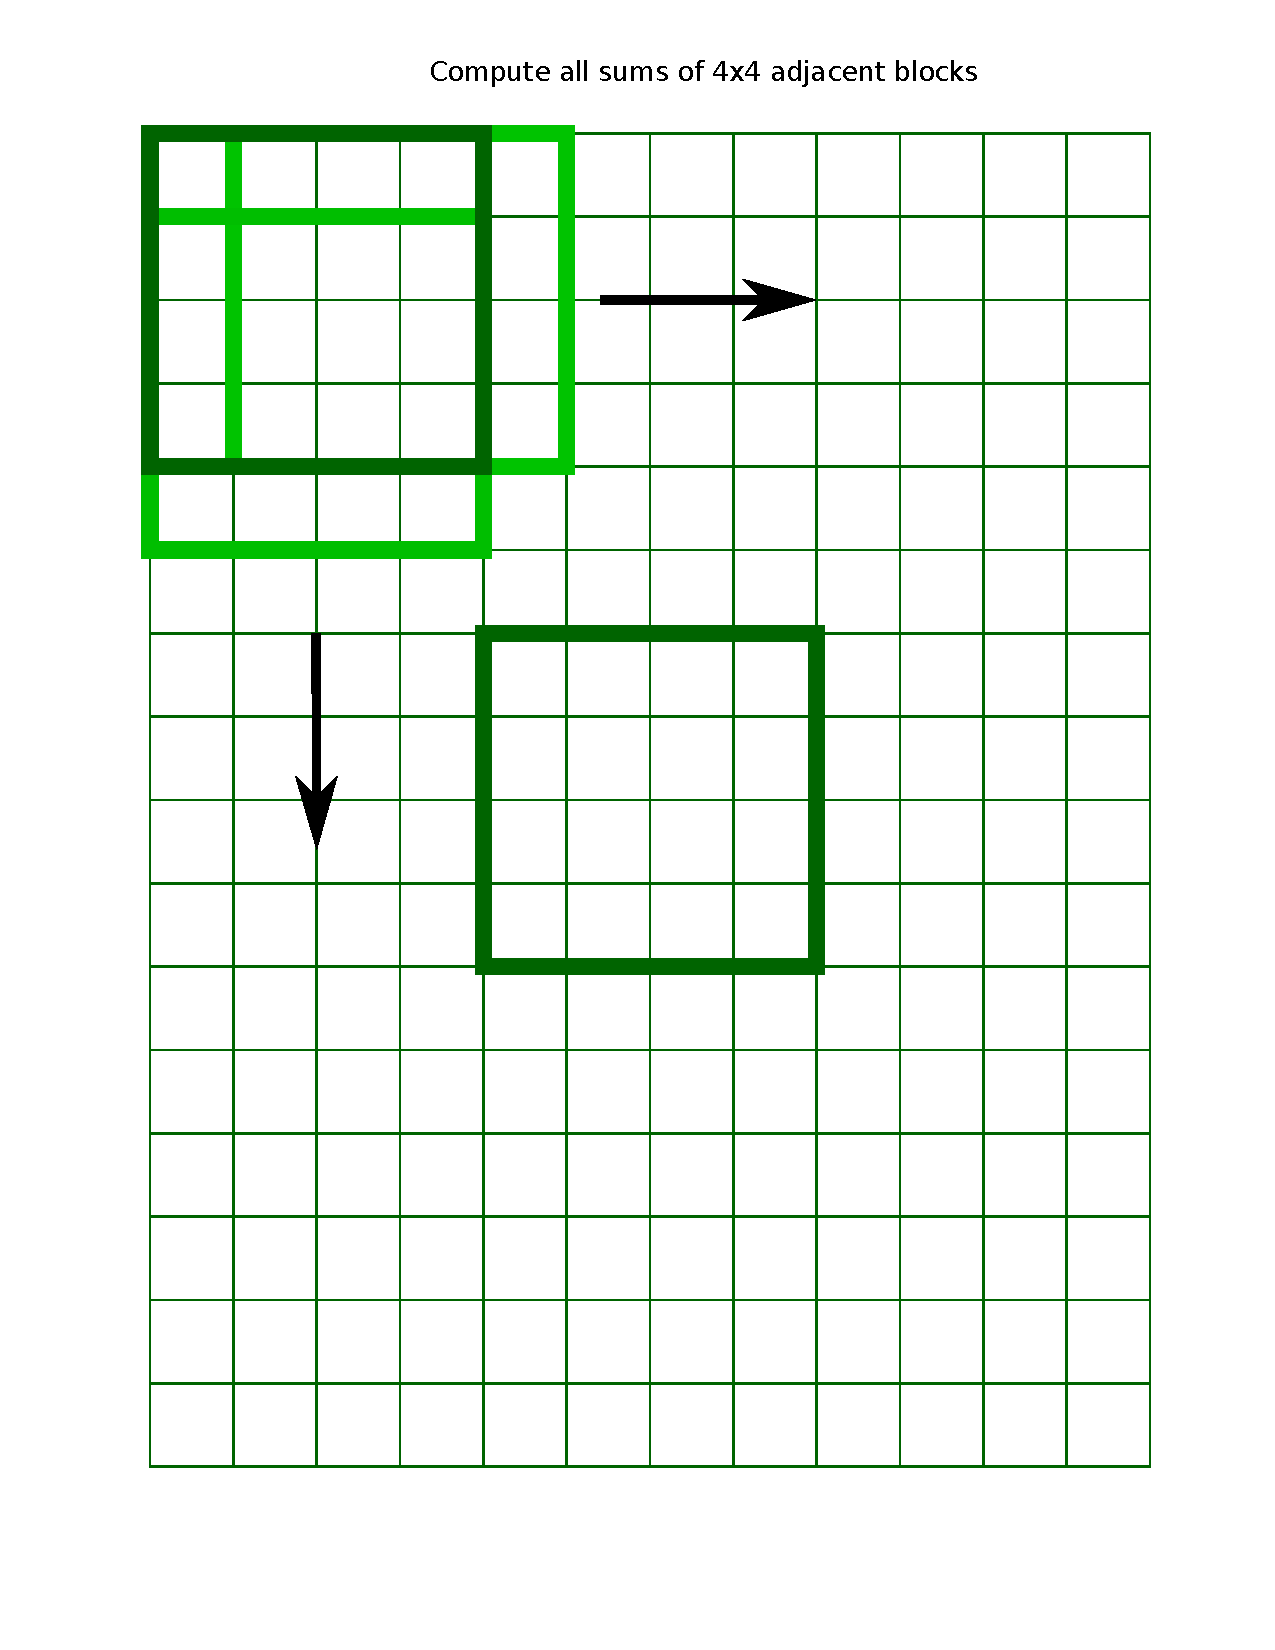
\includegraphics[width=\textwidth]{figs/HCALSum.pdf}
  \caption{All sum of 4x4 are computed, if one is above threshold L2 is generated }
\end{figure}

\begin{figure}
  \centering
  % Requires \usepackage{graphicx}
  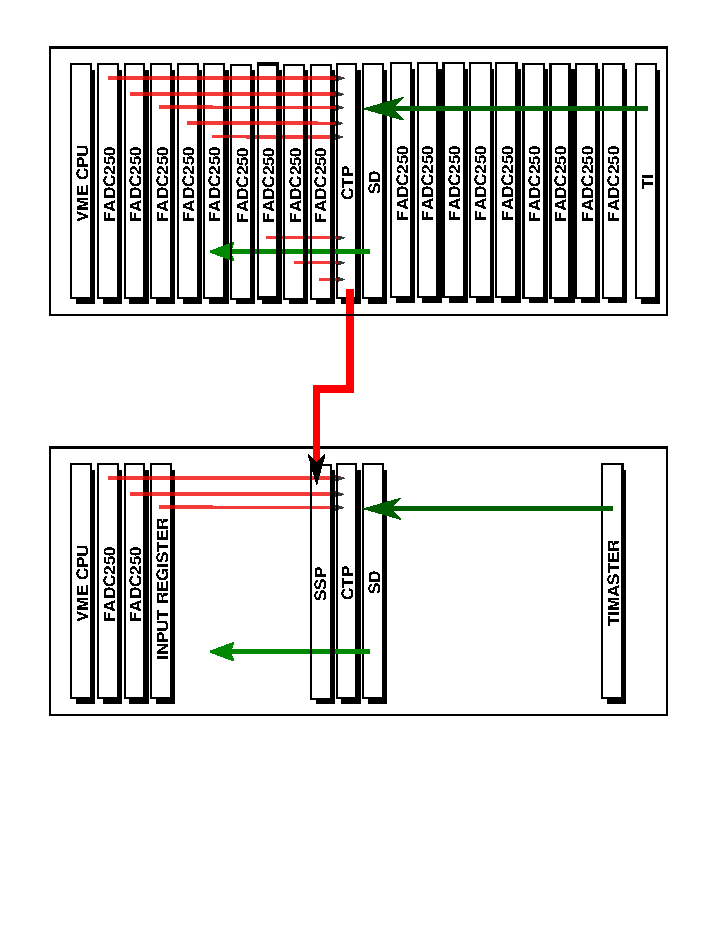
\includegraphics[width=\textwidth]{figs/VXSHCalFADC.pdf}\\
  \caption{HCAL crate layout }\label{fig:HCALFADC}
\end{figure}

\section{Fastbus}
Fastbus is an electronics standard . It can transfer up to 10 Megawords per second with a 32 bit width which gives a maximum theoretical throughput of 40 MB/s which translates in usual sustained rate of 15 MB/s.
Since we have a lot of Fastbus equipment on hand. It will be used in order to save money for the large number of detectors channels. The main readout is the Lecroy ADC 1881M a 13 bit ADC, with a 9 $\mu$s encoding time in 12 bit resolution and 12  $\mu$s. The 1881M features a fast clear and is ready to tahe another event after 1 $\mu$s. For signal requiring time measurement 1877S TDC will be used, they have 96 channels per module. It is multihit with an event buffer of 8 events. It has an encoding time  1.7 $\mu$s plus 50 ns per hit per channel giving a maximum encoding time of 78 $\mu$. 
The Struck Fastbus Interface is a Fastbus Master is controlled by a standard VME controller which allows to control the Fastbus modules through any VME CPU. It is needed in each Fastbus bin to control the Fastbus modules.

\begin{tabular}{|c|c|}
\hline
&\\
\hline
&\\
\hline
\end{tabular}




\section{Detectors}
\subsection{SuperBigBite}
The SuperBigBite spectrometer will be use for several experiments in different configuration. The main elements are a large dipole magnet associated with large GEM trackers to provide the postion of the particles allowing to determine their momentum.
In addtion to the SuperBigBite spectrometer several additionnal detectors will be used.
\subsection{Electron electromagnetic}
The Electromagnetic Calorimeter will have 1920 lead glass blocks arranged in a matrix 60x32 ?. The electromagnetic calorimeter trigger is done by analog summing. 
The front-end system includes 122 custom NIM 2x8 amplifier/summers, 60
4x4 NIM summers, 8 16 chan. NIM discriminators, 9 16 chan. NIM logical OR.
Total of 20 NIM crates for the front-end electronics. Total 2050 RG58 500 ns
cables from the front-end to the DAQ. They would be connected to the 64
BNC-34 patch panels (32 on the front-end side and the same number on the
DAQ side). 
All
The DAQ system includes 12 FastBus crates with 4 power supply units, 12 SFI
modules, 12 CPUs and 12 TI’s, 96 ADCs 1881m and 6 TDCs 1877S.
\subsection{Hadron calorimeter}
This hadronic calorimeter will be used as proton and neutron trigger.
It has 24x12 = 288 channels. The readout and trigger will be done using FADCs.
For the neutron experiment the detector will also give the neutron momentum by measuring the time of flight. In this configuration we plan to split the signal between FADC and discriminator to go to high resolution TDC.
\subsection{Coordinate detector}
The coordinate detector is an array of 2352 thin planes of scintillators readout by multianode PMTs. They will have a front end electronics based on the NINO chips which will give a discriminated signal for all the channels. The logic signals will be fed to Fastbus TDC 1877S. 
\subsection{Big Bite Spectrometer}
The Big Bite spectrometer is part of standard Hall A equipment it is a smaller dipole with a detector stack. 
For the SBS experiment the electron detector stacj will be used.
\subsubsection{Electromagnetic calorimeter}
The main electron trigger is the shower detector. The shower is 7x27 lead glass blocks. An analog sum of 7 blocks is made. This sums are further added using 4 channels linear fan module.
A preshower layer 2x27 is placed in front of the shower but is usually used off line for pion electron identification. This make a total of 189 + 54 = 243 lead glass blocks to be readout.
The readout of the detector will be done using fastbus using ADCs 1881M.
\subsubsection{Scintillator array}
For timing measurement a 90 paddles scintillator array is being build by the Glasgow group, they will be readout by both sides giving 180 channels to be readout. The paddles will be readout using a front end with the NINO chip and send to Fastbus TDC 1877S..
\subsubsection{Gas Cerenkov detector GRINCH}
For the BigBite detector a new highly segment Gas Cerenkov is being built by William and Mary and A\&T University. It will have 550 PMTs channels readout using the NINO front end.
\subsubsection{GEM trackers}
The front trackers of the GeP5 will be fitted to Big Bite to be used as main tracking device improving the rate capablility. It will use the same APV25 with INFN MPD VME readout.
\subsubsection{BigBite electron trigger}
The BigBite electron trigger is based on analog summing usimg sum of 7 blocks
\newpage
\begin{figure}
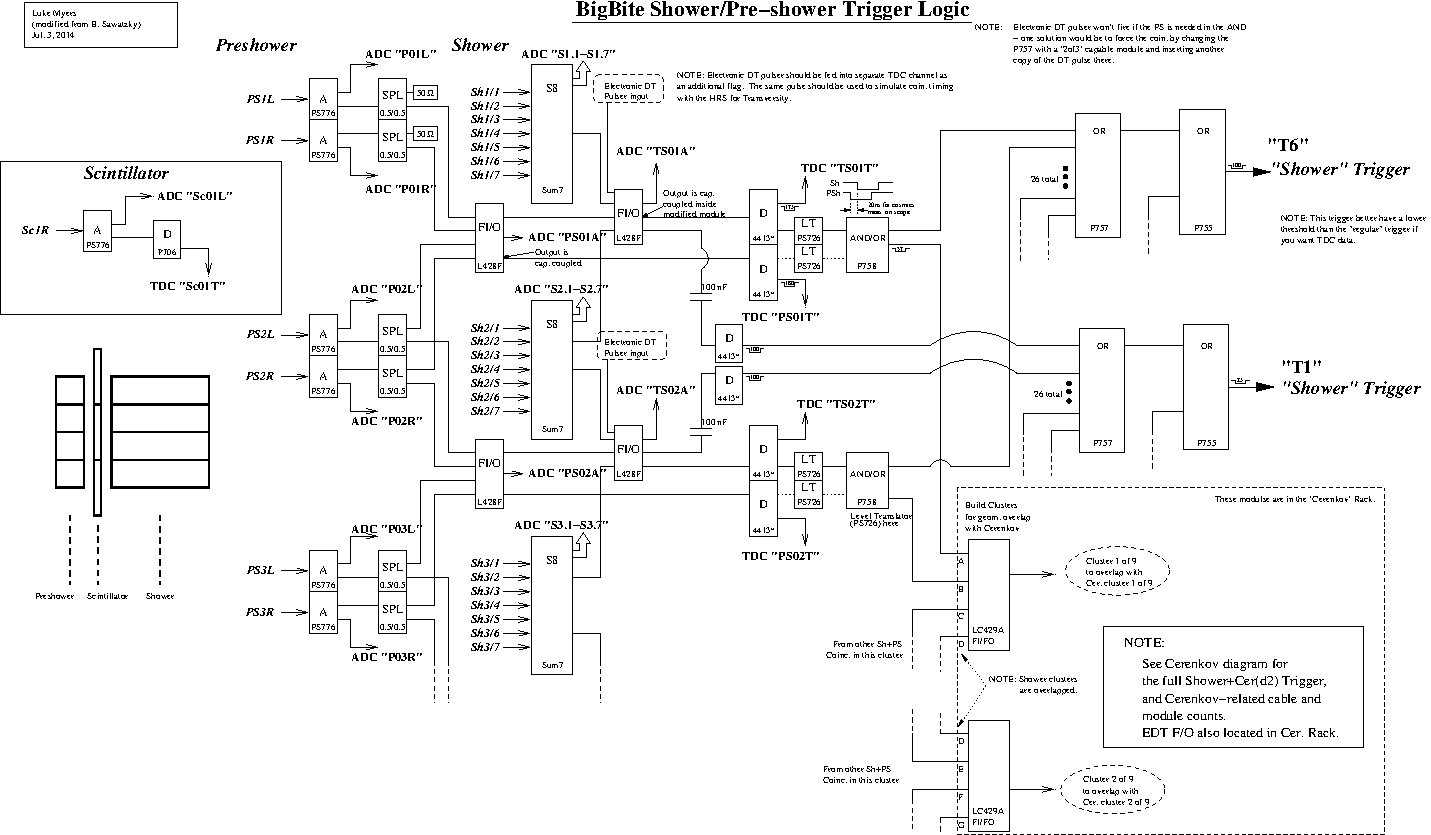
\includegraphics[scale=0.9,angle=270]{figs/Sh-PS_logic_v2A.pdf}\\
\caption {BigBite electron shower analog sum trigger \label{BBEtrig}}
\end{figure}
\newpage
\subsection{HERMES RICH detector}
The INFN HERMES RICH detector was loaned to University of Connecticut for
the transversity experiment. It is a dual radiator RICH
readout with an array of 1934 PMTs. The readout will be done with the NINO chips and 1877S TDCs. 

\subsection{Detector configuration summary}
%\begin{tabular}{|c|c|c|c|c|c|c|}
%\hline
%Experiment&Trigger & Detectors & Subdetectors & Channels& Readout & Type \\
%&rate&&&&&\\
%\hline
%GEp5& 3 KHz  & SBS & Front tracker & 60,000 & APV25 MPD& VME\\ 
% && & Back tracker & 64,000& APV25 MPD& VME\\
% && & HCAL & 288 & FADC 250 &VME\\
% & & Electron arm& ECAL & 1920 & ADCs 1881M&Fastbus\\ 
% &&              & CDET & 2352 & ADCs 1877S &Fastbus \\ 
%\hline
%GEn& 5KHz & SBS & HCAL & 288 & FADC 250 &VME\\ 
% &    &   & CDet & 2352 & ADCs 1877S&Fastbus\\ 
% && BigBite& Shower & 243 & ADCs 1881M&Fastbus\\ 
% && & Scintillator & 180& ADCs 1877S&Fastbus\\ 
% && & Gas Cerenkov & 550& ADCs 1877S&Fastbus\\ 
% && & Front Tracker & 60,000& APV25 MPD &VME\\ 
%\hline
%GMn& 5KHz & SBS & HCAL & 288 & FADC 250 &VME\\ 
%   &  &   & CDet & 2352 & ADCs 1877&Fastbus\\ 
% && BigBite& Shower & 243 & ADCs 1881M&Fastbus\\ 
% && & Scintillator & 180 & ADCs 1877S&Fastbus\\ 
% &&& Gas Cerenkov & 550 & ADCs 1877S&Fastbus\\ 
% &&& Front tracker & 60,000 &APV25 MPD& VME\\ 
%\hline
%Transversity &5KHz& SBS & Back tracker &64,000&APV25 MPD& VME\\
% &&  & RICH & 1934 & ADCs 1877S&Fastbus\\
% &&  & HCAL & 288 & FADC 250 &VME\\ 
% && Big Bite & GRINCH&550 &  ADCs 1877S&Fastbus\\
% &&  & Front tracker & 60,000& APV25 MPD &VME\\
%\hline
%\end{tabular}

%% New table from Mark
\subsection{Detector configuration summary}
\begin{tabular}{|c|c|c|c|}
\hline
GEp Detectors & Channels& Readout & Type \\
\hline
\underline{SBS Proton arm} & & & \\
Front tracker (6 GEM chambers) & 60,000 & APV25 MPD& VME\\
Rear tracker (10 GEM chambers) & 64,000& APV25 MPD& VME\\
HCAL & 288 & FADC 250 &VME\\
\hline
\underline{Electron arm} & & & \\
ECAL & 1920 & ADCs 1881M&Fastbus\\
CDET & 2352 & ADCs 1877S &Fastbus \\
\hline
\hline
GEn/GMn Detectors & Channels& Readout & Type \\
\hline
\underline{SBS Proton arm} & & & \\
HCAL & 288 & FADC 250 &VME\\
CDet & 2352 & ADCs 1877S&Fastbus\\
\hline
\underline{BigBite Electron arm} & & & \\
PreShower/Shower & 243 & ADCs 1881M&Fastbus\\
Scintillator & 180& ADCs 1877S&Fastbus\\
Gas Cerenkov & 550& ADCs 1877S&Fastbus\\
Front Tracker (4 GEM chambers) & 40000& APV25 MPD &VME\\
Rear Tracker (1 GEM chamber) & 40000& APV25 MPD &VME\\
\hline
\end{tabular}




\section{Data acquisition for GEp5 experiment}
\subsection{Requirements}
The main trigger is the electron trigger generated by the calorimeter.
Depending on the threshold we 
\begin{tabular}{|c|c|}
Threshold & Rates\\
\end{tabular}


\subsection{Detectors}



\subsection{Trigger}

We assume a L1 trigger rate of 200 KHz. 

There are 248 groups
of eight when I assume that all blocks are 4x4cm. In reality a mixture
of block size with frontal areas of 3.8x3.8, 4.0x4.0 and 4.2x4.2 will be
used. In the left figure, the groups of 32 blocks are indicated connecting
group of 8 blocks by different colored squares. The group of 32 blocks overlap
by two groups of 8 in both horizontal and vertical directions. So most of the
groups of 8 have to go to 4 groups of 32. At the edges the groups of 8 feed into
two groups of 32. There are 228  groups of 32 are sums of 4 groups of 8 using
a 4 input channel linear FI/FO. The 228 groups of 32 would have to
go into discriminators.

The L1 will be used to trigger the  electronics.

\begin{figure}
  \centering
  % Requires \usepackage{graphicx}
  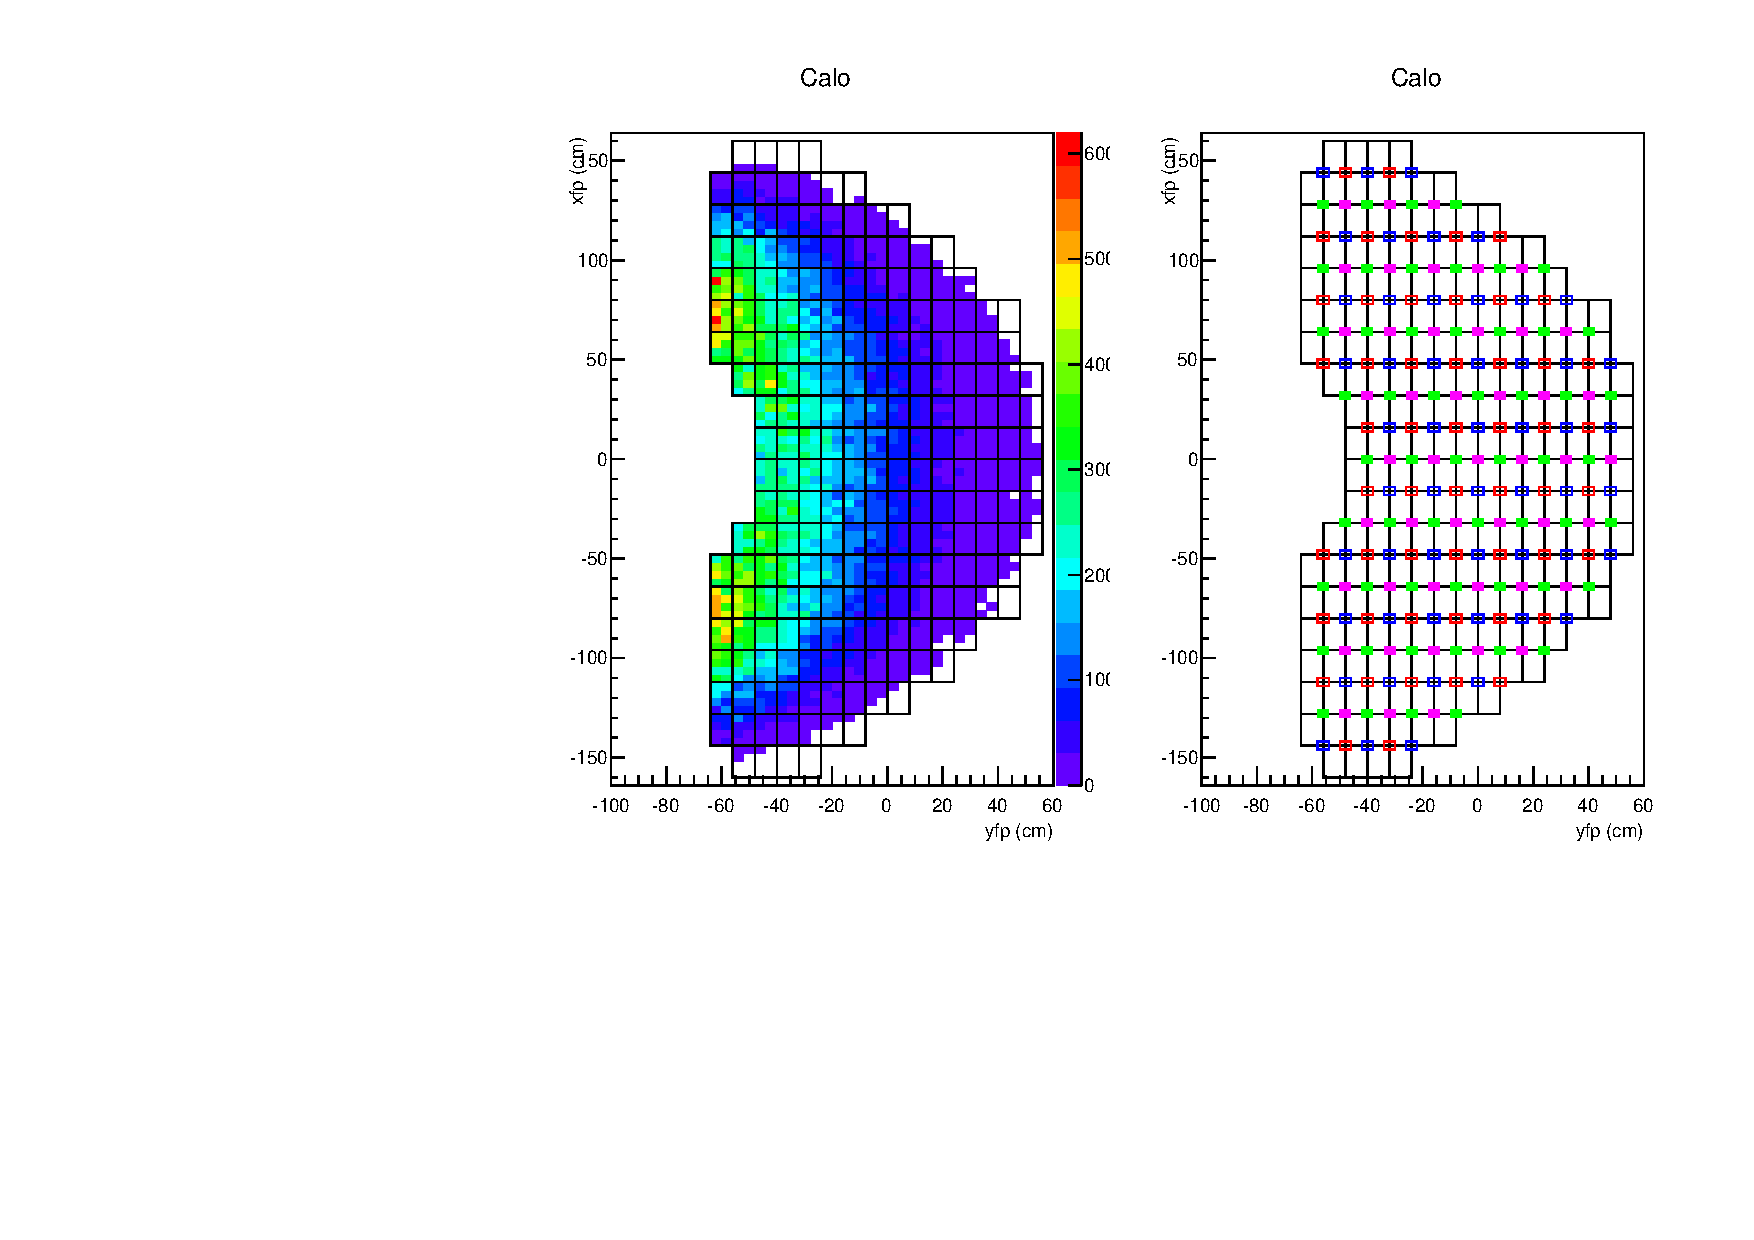
\includegraphics[width=\textwidth]{figs/cfpa.pdf}\\
  \caption{ECAL analog trigger }\label{fig:ECALTrig}
\end{figure}

In parallel the Hadron calorimeter is readout and a proton single trigger will be generated.
The rates expected in the calorimeter


\subsection{Readout}

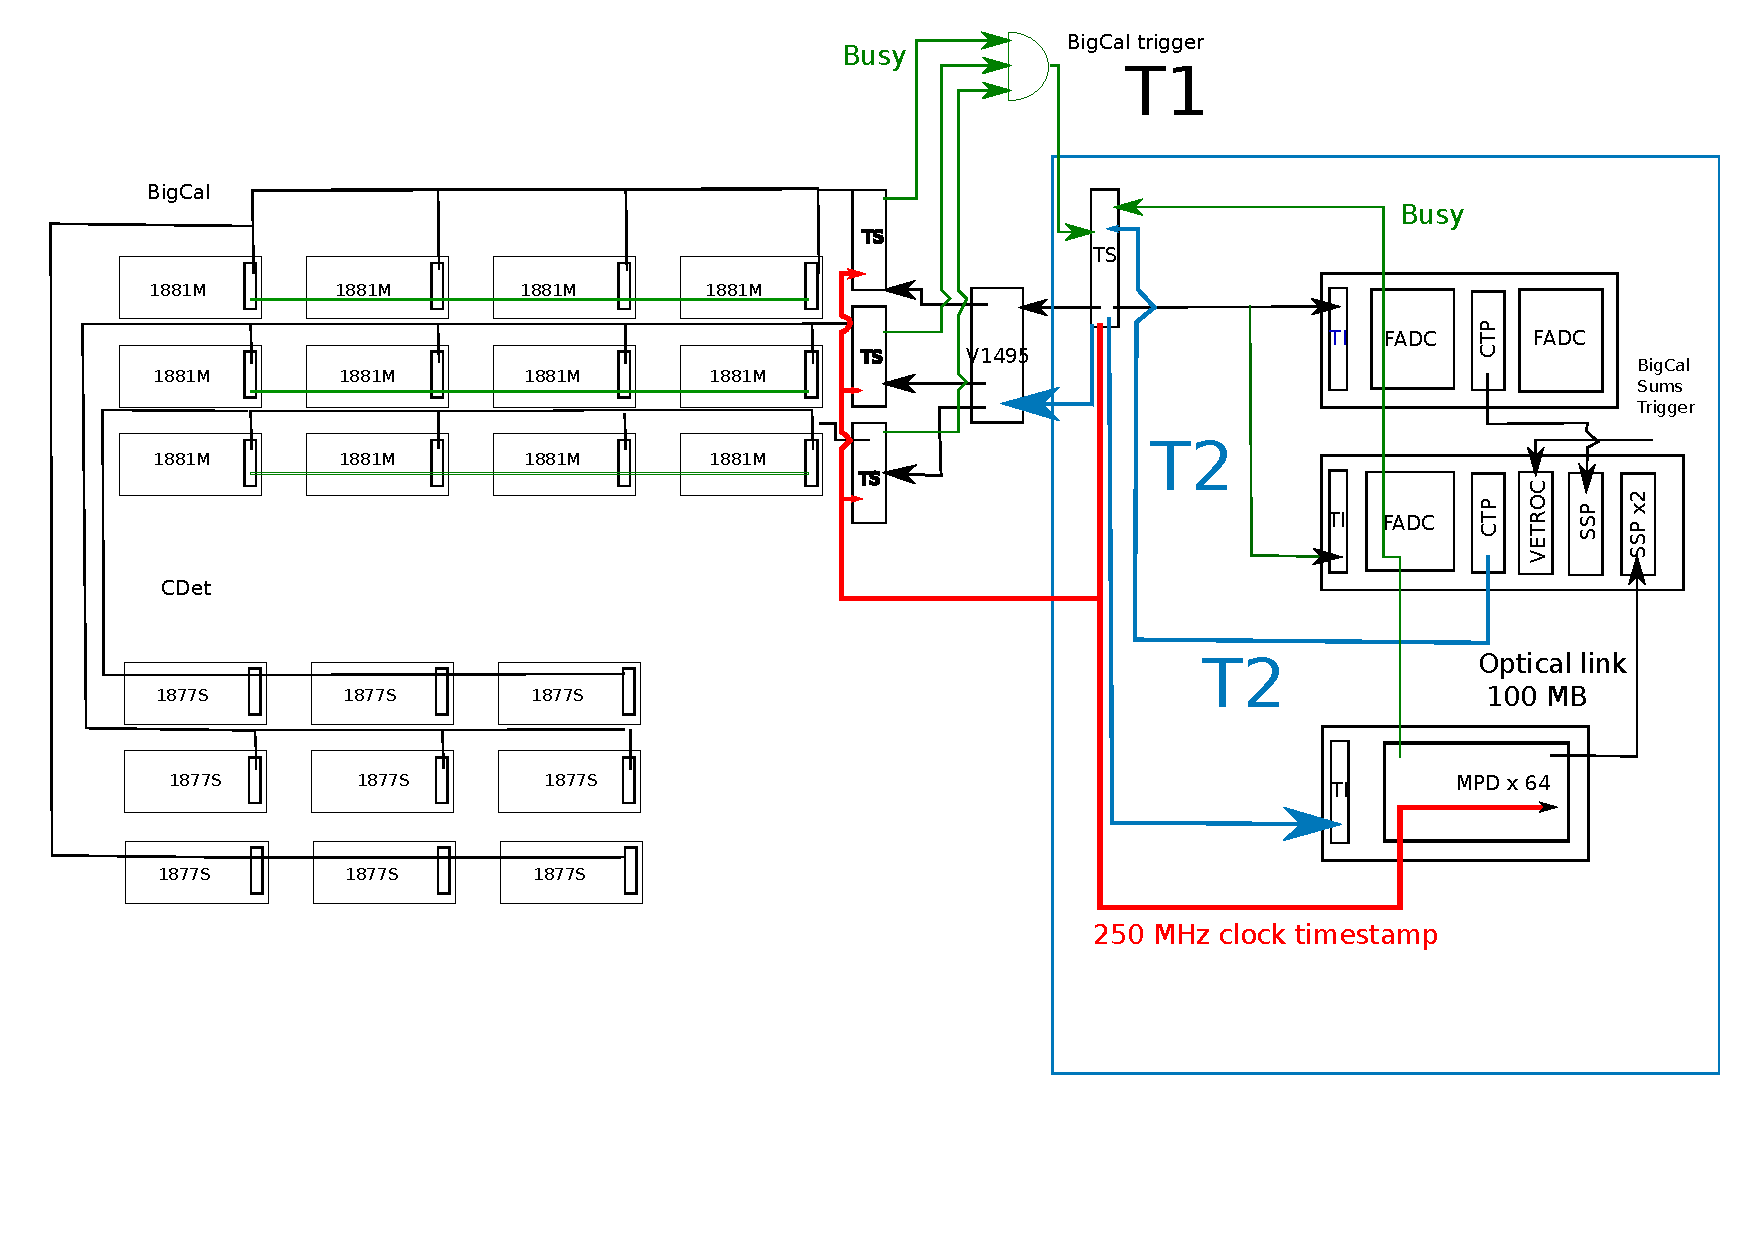
\includegraphics[scale=0.55]{figs/SBSlayoutOld.pdf}\\


\subsection{Event size and data rates}
\section{Data acquisition for GEn experiment}

PR-09-016 GEN
about 2 kHz from a simulation based on pion production rates from a parameterization done by
Wiser [69], Fig. 22. This simulation when compared to the previous Gn
E experiment predicted rates
higher by a factor of 5, so this produces an upper limit on expected rates. Furthermore, adding the
Cerenkov into the trigger configuration to explicitly reject pions and photons will be possible if
necessary


\subsection{Requirements}
\subsection{Detectors}
\subsection{Trigger}
The trigger will be single quasielastic electron in BigBite.
The expected trigger rate at high Q2 is low even without having the Gas Cerenkov in the trigger.
In case of unforeseen background, the same scheme as GEp5 could be used by using a L1 and L2 trigger from HCAL for a neutron trigger
to have a coincidence between the two arms.
\subsection{Readout}

\subsection{Event size and data rates}
\section{Data acquisition for GMn experiment}
Comparing those thresholds
to Fig. 23 shows that the expected background trigger rates are comfortably low, generally well
below 1 kHz.

Q2 3.5 4.5 6.0 8.5 10. 12. 13.5 16. 18.
Quasi-elastic E’min (GeV) 2.4 1.8 1.1 1.8 3.0 2.0 1.4 2.1 1.2
Threshold (GeV) 2.1 1.6 1.0 1.6 2.7 1.8 1.2 1.9 1.0



\subsection{Requirements}
\subsection{Detectors}
The configuration is similar to the GEn experiment except for calibration run using the RHRS.

\subsection{Trigger}

\subsection{Readout}

\subsection{Event size and data rates}

\section{Data acquisition for transversity experiment}
\subsection{Requirements}
This experiment
Beam current of 40 μA
3He target 50 cm long with 11.5 atm pressure, 65\% 3He transverse polarization with
86\% effective neutron polarization

At the proposed luminosity, the upper limit for the hit rate in the Super BigBite tracker
was estimated as 60 kHz/cm2. This is three times higher than the 20 kHz/cm2 obtained
from the MC simulation using code developed for the GEP5 experiment with just the 3He
target cell. We used the factor of 3 to allow for differences with the optimized GEP5 setup
and possible problems in the optimization of the more complicated polarized target setup.
The rate of 60 kHz/cm2 presents no problem for the GEM operation. The expected hit rate
will be about 100 MHz through the whole area of the tracker.
The resulting
rate per PMT will be about 700 kHz. With a 50 ns window time interval relative to the
hadron calorimeter time signal, this rate leads to less than a 5% occupancy in the RICH,
which is a good operational condition. The dead time of the electronics at this rate could
lead to a loss of some of the hits in PMT. It was estimated to be of 7%.
The calorimeter counting rate vs the threshold energy is presented in Fig. 3.8 obtained
from the ”Wiser” code [19]. The counting rate for the threshold of 2 GeV is about 3 MHz,
which means the probability of a second hit in 50 ns time window relative to the electron
time signal will be 15%. The corresponding false tracks will be rejected after a check of the
correlation of its vertex at the target with the electron arm track vertex at the target.


At projected luminosity, the expected hit rate in the BigBite tracker will be less than
30 kHz/cm2. This estimate was obtained by using the observed experimental rate of MWDCs
and a MC prediction for the photon flux at higher beam energy. Such a rate is comfortable
for the GEM tracker which could operate at rate up to 50 MHz/cm2.
The operation of the shower detector is also well understood from our previous experiment
with the BigBite spectrometer. The counting rate of the calorimeter expected in the proposed
experiment is shown in Fig. 3.10. The threshold level of 1 GeV, which is required in this
experiment for lowest x bin, will result in 200 kHz counting rate. The recently constructed
Gas Cherenkov counter will be used for suppression events with non-electron induced trigger
rate . Expected rate of the whole Cherenkov counter due to high energy electrons is of 5 kHz.
The background counting rate of the Gas Cherenkov counter will be suppressed by using a
threshold of 5-6 photo-electrons. Because average number of photo-electrons for good events
expected to be about 18 the efficiency of the counter will be above 98% even for the proposed
high threshold.


\subsection{Detectors}


\subsection{Trigger}
The trigger of the hadron arm will use the signal from the hadron calorimeter with 1.5 GeV
threshold to insure efficient registration of the hadron with momentum above 2 GeV. The
corresponding trigger rate is about 3 MHz, mainly due to hits by the high energy pions.
We will use the trigger of the electron arm, which rate is about 5 kHz, as a DAQ trigger
without on-line coincidence with the hadron arm. If the actual rate of the electron arm
presents problem for DAQ, an additional reduction factor of 6 is possible by requiring a
50 ns coincidence time between the trigger signals of two arms.


\subsection{Readout}

\subsection{Event size and data rates}
\section{A1n}
This experiment is not a SBS experiment but will be the first experiment using BigBite in the
same configuration as for the SBS experiment.

\subsection{Requirements}
\subsection{Detectors}
\subsection{Trigger}

\subsection{Readout}

\subsection{Event size and data rates}
\section{Inventory}

\section{Manpower}

\section{Timeline and milestones}

\section{Budget}
\begin{thebibliography}{9}
\bibitem{GEnProp} PR
\bibitem{GEpProp} PR
\bibitem{GMnProp} PR
\bibitem{TransProp} PR
\end{thebibliography}
\end{document}
